\begin{itemize}
\item[{\textbf{(info)}}]
Power and energy measurement capabilities are necessary to meet the needs of future 
supercomputing power and energy constraints. These mechanisms may differ in implementation 
and purpose and include capabilities for measuring the energy consumption of entire systems, 
platforms (subsystems), cabinets, node, and components.  

\item[{\textbf{(info)}}]
This section is primarily focused on measuring the system power and energy, 
which includes system hardware and software.  

\item[{\textbf{(mandatory)}}]
The vendor shall provide the mechanism, interface, hardware, firmware, software, 
and any other elements that are necessary to capture the individual power and energy measurements. 

\item[{\textbf{(mandatory)}}]
This capability should have no (or minimal and defined) impact on the computation, 
security, and energy consumption of the equipment.  The vendor must describe 
the impact, preferably in quantitative terms.  

\item[{\textbf{(mandatory)}}]
Scalable tools to extract, accumulate, and display power, energy, and temperature 
information (accumulated energy and peak, instantaneous as well as average power 
between any two points in time) should be delivered.

\item[{\textbf{(mandatory)}}]
The power and energy data must be exportable with at least a comma-separated value or 
a user-accessible API. 

\item[{\textbf{(mandatory)}}]
For power, energy (and discrete current and voltage measurements if available) a 
detailed description of the measurement capabilities must be provided, 
including a specified value for measurement precision, accuracy, and how data 
samples are time-stamped. 
WE HAD A LOT OF DISCUSSION ABOUT PRECISION and ACCURACY, 
SHOULD WE EXPAND ON WHAT WE WANT HERE FOR THE ENTIRE DOCUMENT? 
CAN WE PROVIDE A SPECIFIC REQUIREMENT OR BE MORE DESCRIPTIVE ABOUT 
WHAT WE WANT HERE – JHL? Reference ANSI C12.1

\item[{\textbf{(info)}}]
Why hierarchy?

The document is formatted in somewhat of a hierarchical fashion. The purpose of this 
is to address the various current and anticipated future use cases related to this topic. 
Component level measurement, for example, is required for fine-grained application 
power and energy analysis; likewise, component level control could be used to 
shift power from one component to another based on specific application requirements. 
Measurement at node level granularity is necessary for understanding the power and 
energy characteristics of a multi-node application, for example. While cabinet level 
measurement might have fewer current use cases, cabinet level power capping, as well as 
node level, are emerging as important requirements in recent procurements. Platform level 
measurement and control has many facility inspired use cases and is a critical piece of 
overall platform management.

\item[{\textbf{(info)}}]
Reported Values versus Internal Samples

%INCLUDE FIG 3-1 
\begin{figure}[htbp]
\centering
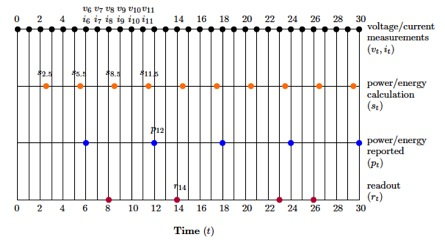
\includegraphics[width=4in]{fig1}
\caption{Power profile HPL run}
\label{fig:powprof}
\end{figure}

A number of terms are used in this document to describe measurement capabilities. 
It is important to understand the context in which the terms are used. 
Figure~\ref{fig:powprof} illustrates these terms. The x-axis of Figure~\ref{fig:powprof} 
is Time (in generic units). Note that Figure~\ref{fig:powprof} represents a range of 
possible capabilities that are useful for this discussion; it does not imply that 
these specific capabilities are a requirement.

\begin{itemize}
\item
The top horizontal line represents points in time when discrete internal current and 
voltage measurements are sampled at the device level. These samples are not necessarily 
exposed externally. At each time interval a voltage and current sample is internally 
measured (v6, i6 pair, for example).  
\item
The second line down represents the points in time when an internal power and/or 
energy calculation is performed. Again, the result is not necessarily exposed externally.
\item
The third line down represents the points in time when a reported value is available to be read 
externally. Each reported value could represent an average power, an instantaneous power, 
or an accumulated energy value, depending on the device capabilities. For example, 
point P12 could simply be the power value calculated at S8.5 or S11.5. P12 could also 
be the average power of points S8.5 and S11.5, or all of the calculated power samples prior to P12. 
P12 could likewise be an accumulated energy value representing any range of power samples 
up to that point in time. The important distinction is the difference between the device's 
internal sampling capability (frequency of and what the samples represent) and the external 
reported value capability of the device (again, frequency of and what the values represent).
\item
Finally, the forth line down represents when the user actually obtains the reported value 
readout. It is critical that the timestamp of the reported value represents the time 
of the measurement as accurately as possible. Note that the actual readout takes place 
at various time intervals following the availability of the reported value. This emphasizes 
the importance of timestamping at the time of measurement, not at the time of reading the value.
\end{itemize}

For example, a measurement device may be capable of producing 100 discrete power 
samples per second (internally). The power calculation (sample) and availability of the 
reported value of this same device may be equivalent to the lowest level sampling frequency, 
but no greater. Both, are typically less than the internal sampling frequency. For example, 
the same device may have the ability of producing a reported a value at 10 times per second. 
This reported value could be a power value averaged over 10 seconds, an accumulated energy value 
that includes 10 additional seconds with each new reported value, or simply a discrete 
(instantaneous) power value for that moment in time. 

Generally speaking, the requirements for the frequency of the reported value depend on 
what the reported value represents. If the reported value is a discrete power value, 
then a higher frequency of reported value is typically desired. If the reported value 
represents an average power or accumulated energy value, reported frequency is less 
important than the internal sampling frequency that is used to derive the reported 
average power or energy value.
\end{itemize}

\section{System, Platform, and Cabinet Level Measurements}

%INSERT TABLE 1
\begin{table}[htbp]
\caption{System, platform, and cabinet requirements for internal and reported frequency}
\label{tab:spclevel}
\begin{tabular}{|p{3.0cm}|p{3.5cm}|p{3.5cm}|p{3.5cm}|} \hline
& & \textbf{Internal Sample}&\textbf{External}\\ 
& & \textbf{Frequency}&\textbf{Reported Value}\\ 
& & & \textbf{Frequency}\\ \hline

\textbf{Mandatory} &
Discrete power (W)&
\mbox{$ \ge $} 1 per second &
\mbox{$ \ge $} 1 per second \\

& 
Average Power (W) &
\mbox{$ \ge $} 10 per second &
\mbox{$ \ge $} 1 per second \\

& 
Energy (J) &
\mbox{$ \ge $} 10 per second &
\mbox{$ \ge $} 1 per second \\ \hline

\textbf{Important} & 
Discrete power (W)&
\mbox{$ \ge $} 10 per second &
\mbox{$ \ge $} 10 per second \\

& 
Average Power (W) &
\mbox{$ \ge $} 100 per second &
\mbox{$ \ge $} 1 per second \\

& 
Energy (J) &
\mbox{$ \ge $} 100 per second &
\mbox{$ \ge $} 1 per second \\ \hline 

\textbf{Enhancing} & 
Discrete power (W)&
\mbox{$ \ge $} 100 per second &
\mbox{$ \ge $} 1000 per second \\

& 
Average Power (W) &
\mbox{$ \ge $} 1000 per second &
\mbox{$ \ge $} 1 per second \\

& 
Energy (J) &
\mbox{$ \ge $} 1000 per second &
\mbox{$ \ge $} 10 per second \\ \hline

\end{tabular}
\end{table}
\begin{itemize}
\item[\textbf{(info)}]
The system level may vary by site and architecture, but could be so broad as to 
include all the parts of the system that explicitly participate in performing 
any workload(s). This might include supporting internal and external power and 
cooling equipment as well as internal and external communication and storage sub-systems. 

\item[\textbf{(info)}]
The platform is distinguished from the system so 
that compute equipement is differentiated from 
other system-level equipment (such as external storage) that may be managed distinctly,
yet together make up a system. 

\item[\textbf{(info)}]
The cabinet (or rack) is the first order discretization of the platform 
level measurement. The cabinet may be part of the compute, storage or networking platform. 

\item[\textbf{(mandatory)}]
Must be able to measure system, platform, and cabinet power and energy.

Table~\ref{tab:spclevel} lists the mandatory, important and enhancing requirements for 
the internal sampling frequency (internal device capability) and the external reported 
value frequency (data available to the consumer) at the system, platform and cabinet level. 
Figure~\ref{fig:powprof} should be referenced in conjunction with Table~\ref{tab:spclevel} to 
help clarify these requirements. Note that Figure~\ref{fig:powprof} also depicts readout, 
i.e. when the consumer chooses to read the data. Readout rate will not be addressed in 
the requirements since readout rate is driven by the computer and limited by the reported 
value frequency. The details describing the internal sampling frequency (voltage and 
current or power) and how the average power and/or energy value is calculated \textbf{must} be provided.

\item[\textbf{(mandatory)}]
The power and energy values must be based on electrical measurements 
(e.g., based on shunts or Hall effect sensors). Values that are derived from 
heuristic models based on architectural events or system state (e.g., RAPL) can 
complement but not replace them.

\item[\textbf{(important)}]
The vendor shall assist in the effort to collect these data in whatever other 
subsystems are provided (e.g., another vendor’s back-end storage system). 

\item[\textbf{(important)}]
Those elements of the system, platform and cabinet that perform infrastructure-type 
functions (e.g., cooling and power distribution), must be measured separately with the 
ability to isolate their contribution to the power and energy measurements.  

\end{itemize}

\section{Node Level Measurements}

%INSERT TABLE 2
\begin{table}[htbp]
\caption{Node Level Requirements for internal and reported frequency}
\label{tab:nodelevel}
\begin{tabular}{|p{3.0cm}|p{3.5cm}|p{3.5cm}|p{3.5cm}|} \hline
& & \textbf{Internal Sample}&\textbf{External}\\ 
& & \textbf{Frequency}&\textbf{Reported Value}\\ 
& & & \textbf{Frequency}\\ \hline

\textbf{Mandatory} &
Discrete power (W)&
\mbox{$ \ge $} 1 per second &
\mbox{$ \ge $} 1 per second \\

& 
Average Power (W) &
\mbox{$ \ge $} 10 per second &
\mbox{$ \ge $} 1 per second \\

& 
Energy (J) &
\mbox{$ \ge $} 10 per second &
\mbox{$ \ge $} 1 per second \\ \hline

\textbf{Important} & 
Discrete power (W)&
\mbox{$ \ge $} 10 per second &
\mbox{$ \ge $} 10 per second \\

& 
Average Power (W) &
\mbox{$ \ge $} 100 per second &
\mbox{$ \ge $} 1 per second \\

& 
Energy (J) &
\mbox{$ \ge $} 100 per second &
\mbox{$ \ge $} 1 per second \\ \hline 

\textbf{Enhancing} & 
Discrete power (W)&
\mbox{$ \ge $} 100 per second &
\mbox{$ \ge $} 1000 per second \\

& 
Average Power (W) &
\mbox{$ \ge $} 1000 per second &
\mbox{$ \ge $} 1 per second \\

& 
Energy (J) &
\mbox{$ \le $} 1000 per second &
\mbox{$ \le $} 10 per second \\ \hline

\end{tabular}
\end{table}

\begin{itemize}

\item[\textbf{(info)}]
A node level measurement shall consist of the combined measurement of all components that 
make up a node for the architecture. For example, components may include the CPU, memory, 
and the network interface. If the node contains other components such as spinning or solid 
state disks they shall also be included in this combined measurement. The utility of the 
node level measurement is to facilitate measurement of the power and energy characteristics 
of a single application. The node may be part of the network or storage equipment, such 
as network switches, disk shelves, and disk controllers.   

\item[\textbf{(important)}]
The ability to measure the power and energy of any and all nodes must/should 
be provided.  NOTE: Should this be mandatory? Change must/should appropriately.

Table~\ref{tab:nodelevel} lists the mandatory, important, and enhancing requirements 
for the internal sampling frequency (internal device capability) and the external 
reported value frequency (data available to the consumer) at the node level. Figure~\ref{fig:powprof}
should be referenced in conjunction with Table~\ref{tab:nodelevel} to help clarify 
these requirements. Note that Figure~\ref{fig:powprof} also depicts readout, i.e., when 
the consumer chooses to read the data. Readout rate will not be addressed in the 
requirements since readout rate is driven by the computer and limited by the reported 
value frequency. The details describing the internal sampling frequency (voltage and 
current or power)and how the average power and/or energy value is calculated \textbf{must} be provided.

\item[\textbf{(mandatory)}]
The power and energy values must be based on electrical measurements (e.g., based on shunts 
or Hall effect sensors). Values that are derived from heuristic models based on 
architectural events or system state (e.g., RAPL) can complement but not replace them.
\end{itemize}


\section{Component Level Measurement}

%INSERT TABLE 3
\begin{table}[htbp]
\caption{Component Level Requirements for internal and reported frequency}
\label{tab:comlevel}
\begin{tabular}{|p{3.0cm}|p{3.5cm}|p{3.5cm}|p{3.5cm}|} \hline
& & \textbf{Internal Sample}&\textbf{External}\\ 
& & \textbf{Frequency}&\textbf{Reported Value}\\ 
& & & \textbf{Frequency}\\ \hline

\textbf{Mandatory} &
Discrete power (W)&
\mbox{$ \ge $} 1 per second &
\mbox{$ \ge $} 1 per second \\

& 
Average Power (W) &
\mbox{$ \ge $} 10 per second &
\mbox{$ \ge $} 1 per second \\

& 
Energy (J) &
\mbox{$ \ge $} 10 per second &
\mbox{$ \ge $} 1 per second \\ \hline

\textbf{Important} & 
Discrete power (W)&
\mbox{$ \ge $} 10 per second &
\mbox{$ \ge $} 10 per second \\

& 
Average Power (W) &
\mbox{$ \ge $} 100 per second &
\mbox{$ \ge $} 1 per second \\

& 
Energy (J) &
\mbox{$ \ge $} 100 per second &
\mbox{$ \ge $} 1 per second \\ \hline 

\textbf{Enhancing} & 
Discrete power (W)&
\mbox{$ \ge $} 100 per second &
\mbox{$ \ge $} 1000 per second \\

& 
Average Power (W) &
\mbox{$ \ge $} 1000 per second &
\mbox{$ \ge $} 1 per second \\

& 
Energy (J) &
\mbox{$ \le $} 1000 per second &
\mbox{$ \le $} 10 per second \\ \hline

\end{tabular}
\end{table}
\begin{itemize}

\item[\textbf{(info)}]
Components are the physically discrete units that comprise the node. This level of measurement 
is important to analyze application energy/performance trade-offs. This level is analogous 
to performance counters and carries many of the same motivations.  Components may not 
only be silicon devices.  For example, it would be useful to know how much fan energy is 
being used by the Muffin fans at the back of the rack or by some active rear door cooling 
methodology.  Also, some systems may have a cabinet power distribution unit (CDU).  How 
much energy is being used by the CDU for motors, fans.
	
\item[\textbf{(enhancing)}]
The ability to measure the power and energy of each individual component must 
(or should if this is enhancing?) be provided.
	
Table~\ref{tab:comlevel} lists the mandatory, important, and enhancing requirements for 
the internal sampling frequency (internal device capability) and the external reported value 
frequency (data available to the consumer) at the node level. Figure~\ref{fig:powprof} should 
be referenced in conjunction with Table~\ref{tab:comlevel} to help clarify these requirements. 
Note that Figure~\ref{fig:powprof} also depicts readout, i.e., when the consumer chooses to 
read the data. Readout rate will not be addressed in the requirements since readout rate 
is driven by the computer and limited by the reported value frequency. The details describing 
the internal sampling frequency (voltage and current or power) and how the average 
power and/or energy value is calculated \textbf{must} be provided.

\item[\textbf{(mandatory)}]
The power and energy values must be based on electrical measurements (e.g., based on 
shunts or Hall effect sensors). Values that are derived from heuristic models based 
on architectural events or system state (e.g., RAPL) can complement but not replace them.
\end{itemize}


